\documentclass[a4paper,11pt]{article}
\usepackage[big]{layaureo}
\usepackage[T1]{fontenc}
\usepackage[utf8]{inputenc}
\usepackage[british,UKenglish,USenglish,english,american]{babel}
\usepackage{textcomp}
\usepackage{amsmath}
\usepackage{dsfont}
\usepackage{amssymb}
\usepackage{graphicx}
\usepackage{multirow}
\usepackage{caption}
  \captionsetup{format=hang,labelfont=bf,textfont=it, font=small}
\usepackage{subcaption}
  \captionsetup[sub]{position=top}
  \captionsetup[sub]{font=footnotesize}
  \captionsetup[sub]{labelfont={bf,sc}}
\usepackage{booktabs}
\usepackage{tabularx}
\usepackage{siunitx}
\usepackage{color}
\usepackage{fancyhdr}
\usepackage{float}
\usepackage{comment}
\usepackage{verbatim}
\usepackage{braket}
\usepackage[dvipsnames]{xcolor}
%\usepackage[style=verbose, backend=bibtex]{biblatex}
%\bibliography{references}
\usepackage[title]{appendix}
\usepackage[breaklinks]{hyperref}

\usepackage{listings}

\definecolor{light-gray}{gray}{.95}
\lstset{frame=tb,
  aboveskip=3mm,
  belowskip=3mm,
  showstringspaces=false,
  columns=fullflexible,
  keepspaces=true,
  numbers=left,
  basicstyle={\footnotesize\ttfamily},
  numberstyle=\tiny\color{darkgray},
  keywordstyle=\color{NavyBlue},
  stringstyle=\color{Orange},
  commentstyle=\color{OliveGreen},
  breaklines=true,
  breakatwhitespace=true,
  tabsize=4,
  backgroundcolor=\color{light-gray}
}

\pagestyle{fancy}
\fancyhf{}
\lhead{Federico Agostini, Federico Bottaro}
\chead{\thepage}
\rhead{05/04/2020}
\lfoot{Exam}
\cfoot{\MakeUppercase{Information Theory and Computation}}
\rfoot{2019-2020}

\begin{document}

\title{Implementation of ground state search via Neural Network}
\author{Federico Agostini, Federico Bottaro}
\date{05/04/2020}
\maketitle


\begin{abstract}

The search for the ground state of a many-body system in physics is a topic in which different approach can be implemented. The birth and development of artificial neural networks in the last years has meant that the many-body problem can be treated with this new concepts. We have that a quantum state can be represented by a neural network \cite{Carleo_2017}. In this work, a reinforcement-learning approach is used to train the network and to extract the ground state energy of a given system. The algorithm is evaluated over 1-D and 2-D transverse-field Ising model. A Lanczos algorithm is used to compare the results of the applications.

\end{abstract}

%%%%%%%%%%%%%%%%%%%%%%%%%%%%%%%%%%%%%%%%%%%%%%%%%%
%%%%%%%%%%%%%%%%%%%%%%%%%%%%%%%%%%%%%%%%%%%%%%%%%%
%%%%%%%%%%%%%%%%%%%%%%%%%%%%%%%%%%%%%%%%%%%%%%%%%%

\section{Introduction}

In the field of statistical physics, the behaviour of a complex quantum system can be mimicked using NN such as Restricted Boltzman Machines (RBMs). 

A RBM is a particular type of NN in which the bipartite structure is exploited to extract correlation between the visible units (that represent our data) and the internal representation of the data given by the hidden neurons. In the context of statistical physics RBM's can be seen as a particular ansatz for the many-body wave function. To train our NN we can exploit a reinforcement learning approach in which a set of configuration representing the system can be sampled with numerical approaches like quantum Monte Carlo methods.

The goal of this document is evaluating the ground state of a many body system; hence the starting point is the wave function and its representation. Consider a quantum system with $N$ particles, for examples spins, $\mathcal{S}=(s_1,s_2,\dots,s_N)$. The many-body wave function is a mapping of the $N$-dimensional set $\mathcal{S}$ to complex numbers which fully specify the quantum state. In our context, we want to approximate this black box with a RBM trained to represent $\Psi(\mathcal{S})$.

Focusing on a spin-1/2 quantum system, the visible layer of the RBM is composed by $N$ nodes that corresponds to the physical spins in the chosen basis (in the following $\mathcal{S} = \sigma_1^z \dots \sigma_N^z$), whereas the hidden layer has $M$ auxiliary variables. The quantum states is then described by the expression:
\begin{equation}
    \centering
    \Psi_M(\mathcal{S},\mathcal{W})= \sum _{\{h_i\}} e^{\sum _j a_j \sigma_j ^z + \sum _i b_i h_i + \sum _{ij} W_{ij} h_i \sigma_j ^z},
\end{equation}
where $h_i=\{-1,1\}$ is a set of $M$ hidden units and $\mathcal{W}=\{a_i,b_j,W_{ij}\}$ is the vector of the weights of the network; given an input, they fully specify the response of the network itself. 
\\
Exploiting the absence of intra-layer connection, we can trace out the hidden variables from the wave function and rewrite it as:
\begin{equation}
    \label{eq:Psi_M}
    \centering
    \Psi_M(\mathcal{S},\mathcal{W})= e^{\sum _i a_i \sigma_i ^z} \times  \prod _{j=1}^M 2 \cosh [b_j + \sum_i W_{ij} \sigma_i^z ]
\end{equation}

Since our goal is to evaluate the ground state energy of the system, reinforcement learning proceeds minimizing the expectation value of the energy: $E(\mathcal{W})= \braket{\Psi_M | \mathcal{H} | \Psi _M} / \braket{\Psi_M | \Psi_M}$ with respect to the network weights. In the stochastic setting, this is achieved with an iterative scheme. At each iteration t, a Monte Carlo sampling of $|\Psi_M (\mathcal{S}, \mathcal{W})|^2$ is realized, for a given set of parameters $\mathcal{W}$. At the same time, stochastic estimates of the energy gradient are acquired. In order to obtain an optimal solution for which $\nabla E^* = 0$, Stochastic Reconfiguration (SR) method is used \cite{Sorella}.

The implementation of the algorithm is done both with Fortran and Python. The idea behind the code was the same and the functions are tested with both programming languages, in order to evaluate their correctness. For some numerical instability we can present here results obtained only with the Python script. For more detail see Sec.~\ref{sec:test}.

%%%%%%%%%%%%%%%%%%%%%%%%%%%%%%%%%%%%%%%%%%%%%%%%%%
%%%%%%%%%%%%%%%%%%%%%%%%%%%%%%%%%%%%%%%%%%%%%%%%%%
%%%%%%%%%%%%%%%%%%%%%%%%%%%%%%%%%%%%%%%%%%%%%%%%%%

\section{Theoretical overview of SR}

To reach the goal of finding the ground state energy of a hamiltonian, an iterative procedure is exploited. At each iteration, the value of $\Psi_M$ can be evaluated given the current state of the RBM described by the network parameters $\mathcal{W}$. At the same time, we can sample spin configurations based on $|\Psi_M (\mathcal{S}, \mathcal{W})|^2$, using a Metropolis algorithm. Then the weights of the network are updated using these stochastic estimates, and the process is repeated until convergence.

As marked out in Appendix A of Science 355, 602 (2017) \cite{Carleo_2017}, SR weights update at iteration $p$ is:
\begin{equation}
    \label{eq:update}
    \centering
    \mathcal{W}(p+1)= \mathcal{W}(p) - \lambda(p) S^{-1}(p) F(p)
\end{equation}
where $\lambda$ is the learning rate, $S$ is the covariance matrix
\begin{equation}
    \label{eq:cov_mat}
    \centering
    S_{kk'}(p)= \langle \mathcal{O}^*_k \mathcal{O}_{k'} \rangle -\langle \mathcal{O}^*_k \rangle \langle \mathcal{O}_{k'} \rangle
\end{equation}
and $F$ the forces vector
\begin{equation}
    \label{eq:forces}
    \centering
    F_{k}(p)= \langle E_{loc} \mathcal{O}^*_k  \rangle -\langle E_{loc} \rangle \langle \mathcal{O}_{k'} \rangle.
\end{equation}

The previous equation introduces two important quantity. The term $\mathcal{O}_k$ is a vector containing the variational derivatives of $\Psi_M(\mathcal{S})$ with respect to the $k$-th network parameter $\mathcal{W}_k$. Exploiting the description of the wave function of the RBM (Eq.~\ref{eq:Psi_M}) we can explicitly write the components of the vector $\mathcal{O}_k$ as:
\begin{align}
    \centering
    \label{eq:dPsi_dai}
    \frac{1}{\Psi_M(\mathcal{S})} \partial _{a_i} \Psi_M(\mathcal{S}) &= \sigma _i ^z, \\
    \label{eq:dPsi_dbj}
    \frac{1}{\Psi_M(\mathcal{S})} \partial _{b_j} \Psi_M(\mathcal{S}) &= \tanh[\theta_j (\mathcal{S})], \\
    \label{eq:dPsi_dwij}
    \frac{1}{\Psi_M(\mathcal{S})} \partial _{W_{ij}} \Psi_M(\mathcal{S}) &= \sigma _i ^z \tanh[\theta_j (\mathcal{S})].
\end{align}
%
Above we introduced the effective angles, which correspond to
\begin{equation}
    \theta_j(\mathcal{S})=  b_j + \sum_i W_{ij} \sigma_i^z.
\end{equation}
%
Eq.~\ref{eq:dPsi_dai}, \ref{eq:dPsi_dbj} and \ref{eq:dPsi_dwij} produce respectively $N$, $M$ and $N \times M$ terms.

The second term, introduced in Eq.~\ref{eq:forces}, is the local energy
\begin{equation}
    \label{eq:Eloc}
    \centering
    \begin{split}
    E_{loc} (\mathcal{S}) &= \frac{\braket{\mathcal{S} | \mathcal{H} | \Psi_M}}{\braket{\mathcal{S} | \Psi_M}} \\ 
    %
    &= \sum_{\mathcal{S}'} \frac{\braket{\mathcal{S} | \mathcal{H} | \mathcal{S}'} \braket{\mathcal{S}' | \Psi_M}}{\braket{\mathcal{S} | \Psi_M}} \\
    %
    &= \sum_{\mathcal{S}'} \frac{\braket{\mathcal{S} | \mathcal{H} | \mathcal{S}'} \Psi_M(\mathcal{S}')}{\Psi_M(\mathcal{S})}
    \end{split}
\end{equation}
%
where we applied a completeness relation.

\begin{comment}
From a practical point of view we have that exploiting the RBM description we can write the product:
\begin{equation}
    \centering
    <\mathcal{S} | \Psi_M> = e^{\sum _i a_i \sigma_i ^z} \times  \prod _{j=1}^M 2 cosh [b_j + \sum_i W_{ij} \sigma_i^z ]
\end{equation}

and get an explicit value but in the definition of the local energy we have the term $<\mathcal{S}|\mathcal{H}|\Psi_M>$ that doesn't have an explicit expression. To solve this problem we introduce a 
completeness relation $<\mathcal{S}|\mathcal{H}|\Psi_M> = \sum_{\mathcal{S}'}> <\mathcal{S}|\mathcal{H}|\mathcal{S}'> <\mathcal{S}'|\Psi_M> $ and now we can map a given configuration of $\{+1-1\}$ of dimension $N$ into the Hilbert space of the hamiltonian of dimension $2^N \times 2^N$. 
\end{comment}


To sample spin configurations accordingly to the state of the RBM, Metropolis algorithm is used. Starting from a random configuration $\mathcal{S}$ we flip a spin at random and the new configuration is accepted according to the probability:
\begin{equation}
    \label{eq:Metropolis}
    \centering
    A(\mathcal{S}^k \rightarrow \mathcal{S}^{k +1}) = \min \left(1, \left| \frac{\Psi_M (\mathcal{S}^{k+1})}{\Psi_M (\mathcal{S}^k)} \right|^2 \right).
\end{equation}

%%%%%%%%%%%%%%%%%%%%%%%%%%%%%%%%%%%%%%%%%%%%%%%%%%
%%%%%%%%%%%%%%%%%%%%%%%%%%%%%%%%%%%%%%%%%%%%%%%%%%
%%%%%%%%%%%%%%%%%%%%%%%%%%%%%%%%%%%%%%%%%%%%%%%%%%

\section{Theoretical overview of the Lanczos algorithm}
\label{sec:Lanczos}

Given an hermitian matrix $A$ of size $n\times n$ and a number of iteration $m$, the Lanczos algorithm provide as output a matrix $T$, that is tridiagonal and symmetric with dimension $m \times m$. It holds that $T = V^*AV$, where $V$ is a matrix with orthonormal columns of size $n \times m$. 

The iterative procedure starts from a normalized random vector $v_1$ of size $n$. The fist iteration of the algorithm proceed as follow:
\begin{itemize}
    \item $w_1' = A v_1$
    \item $\alpha _1 = w_1'^* \cdot v_1$
    \item $w_1 = w_1' -\alpha _1 v_1$
\end{itemize}
and then we can start with the iterative procedure for $j=2,\dots ,m$:
\begin{itemize}
    \item $\beta _j = \| w_ {j-1}\|$
    \item $v_j = w_{j-1} / \beta _j $ if $\beta _j \neq 0$ otherwise restart from an arbitrary normalized vector
    \item $w_j ' = A v_j$
    \item $\alpha_j = w_j'^* \cdot v_j$
    \item $w_j = w_j' - \alpha _j v_j - \beta_j v_{j-1} $
\end{itemize}
%
At the end we have that the tridiagonal matrix $T$ has a diagonal composed by the $m$ terms $\alpha_j$ and the off diagonal made up by the $m-1$ terms $\beta_j$. It is possible to demonstrate that the matrix $V$, which satisfies the equation $T = V^*AV$, has the columns that correspond to the $v_1, \dots ,v_m$ vectors.

Since we are interested in the eigenvalues of a given hermitian matrix $A$, we exploit the Lanczos algorithm and evaluate the eigenvalues of the matrix $T$: in fact, $A$ and $T$ have the same eigenvalues, and there are establed procedure to extract this information from a tridiagonal one.

%%%%%%%%%%%%%%%%%%%%%%%%%%%%%%%%%%%%%%%%%%%%%%%%%%
%%%%%%%%%%%%%%%%%%%%%%%%%%%%%%%%%%%%%%%%%%%%%%%%%%
%%%%%%%%%%%%%%%%%%%%%%%%%%%%%%%%%%%%%%%%%%%%%%%%%%

\section{Code development}

The implementation of the algorithm is achieved both in Fortran and in Python. The reason behind that is to have a double check on the correctness of the functions. Moreover, Fortran code does not produce stable results, even if every single routine is tested against the corresponding one in Python and produces the same output given identical inputs (more on these tests can be found in Sec.~\ref{sec:test}).

In the following, the description takes as example the Fortran code, but in Python functions have same names and logic. The references to the listings with the full code can be found in Appendix~\ref{appendix:code}. Results in Sec.~\ref{sec:results} however are obtained with the latter one, due to the problem mentioned above.

%%%%%%%%%%%%%%%%%%%%%%%%%%%%%%%%%%%%%%%%%%%%%%%%%%

\subsection{RBM initialization}
This subroutine randomly initializes the parameters of the RBM, sampling from a normal distribution with mean and standard deviation specified by the user. For more information see Lst.~\ref{lst:RBM_init}.

%%%%%%%%%%%%%%%%%%%%%%%%%%%%%%%%%%%%%%%%%%%%%%%%%%

\subsection{Metropolis simulation}
\label{sec:Metropolis}

The subroutine \texttt{Metropolis} in file \texttt{simulation.f90} deals with the generation of spin configurations given the state of the RBM (expressed by the current values of the weights $\mathcal{W}$). The description of the parameters can be found in Lst.~\ref{lst:Metropolis}, along with the full code. 

\paragraph{Inputs}
The subroutine requires the RBM parameters (one array for the biases of the visible units, one for the hidden and the matrix of the weights between the two) and how many elements we want to save in the output.

\paragraph{Outputs}
The outputs are the sampled spin configurations, saved one per row in a matrix and the vectors of the variational derivatives (Eq.~\ref{eq:dPsi_dai}, \ref{eq:dPsi_dbj}, \ref{eq:dPsi_dwij}), saved in a matrix, one per row.

\paragraph{Description}
Starting from a random configuration (generated by \texttt{Random\_Configuration} subroutine in file \texttt{random.f90}), a random spin is flipped. The new configuration is accepted according to Eq.~\ref{eq:Metropolis}. \\
The calculus of $\Psi_M$ following Eq.\ref{eq:Psi_M} involves exponentials and products, and then leads to overflow problems that affects the acceptance ratio. Since we always deal with ratios of these quantities, the implementation uses logarithms to avoid numerical instabilities; in fact it is possible to write:
\begin{equation}
    \centering
    r = \left| \frac{\Psi_M (\mathcal{S}^{k+1})}{\Psi_M (\mathcal{S}^k)} \right|^2
      = \left| \exp \left[ \log  \Psi_M (\mathcal{S}^{k+1}) - \log \Psi_M (\mathcal{S}^k) \right]\right|^2.
\end{equation}
%
Seeing that $\log \Psi_M(\mathcal{S}) = \sum_i a_i \sigma^z_i + \sum_j \log \left( 2 \cosh \theta_j(\mathcal{S}) \right)$, we get:
\begin{multline}
    \log  \Psi_M (\mathcal{S}^{k+1}) - \log \Psi_M (\mathcal{S}^k) = \\
    = \sum_i a_i(\sigma^z_{i, k+1} - \sigma^z_{i, k}) + \sum_j \log \left[ 2 \cosh \theta_j(\mathcal{S}^{k+1}) \right] - \sum_j \log \left[ 2 \cosh \theta_j(\mathcal{S}^k) \right],
\end{multline}
%
that is what the function \texttt{logPsiDiff} returns (Lst.~\ref{lst:logPsiDiff}).\\
This process is repeated a number of times equal to the input variable \texttt{iter}; the user can also specified the number of iteration to discard before saving the results (through \texttt{burnin}) and the number of steps to wait before two successive records (\texttt{autocorr}), in order to reduce the autocorrelation between the sampled configurations.

%%%%%%%%%%%%%%%%%%%%%%%%%%%%%%%%%%%%%%%%%%%%%%%%%%

\subsection{Covariance Matrix}

Function \texttt{Skk} (Lst.~\ref{lst:Skk}) computes the covariance matrix of Eq.\ref{eq:cov_mat} and applies a regularization since $S_{kk'}$ could be non invertible.

\paragraph{Inputs}
The matrix containing the variational derivatives of $\Psi_M$ given as output from the \texttt{Metropolis} subroutine and the current iteration of the weights update (in order to apply the regularization) are required.

\paragraph{Output}
The output is a \texttt{DOUBLE COMPLEX} matrix describing Eq.~\ref{eq:cov_mat}.

\paragraph{Description}
The final matrix is composed by $S_{kk'}$ plus a regularization term $\lambda(p) = \max(\lambda_0 b^p, \lambda_{min})$ on the diagonal terms. Following \cite{Carleo_2017}, we set $\lambda_0 = 100$, $b=0.9$, $\lambda_{min} = 10^{-4}$, while $p$ is the weights update iteration. In order to avoid numerical problems, every element with absolute value lower than $10^{-9}$ is fixed to 0.

%%%%%%%%%%%%%%%%%%%%%%%%%%%%%%%%%%%%%%%%%%%%%%%%%%

\subsection{Local energy}
\label{sec:LocalEnergy}

At each spin configuration $\mathcal{S}$ can be associated a local energy as delineated in Eq.~\ref{eq:Eloc}. The function \texttt{LocalEnergy} in Lst.~\ref{lst:LocalEnergy} computes this quantity for each configuration generated by the Metropolis algorithm, given the hamiltonian of the system.

\paragraph{Inputs}
This function requires the configuration matrix given as output from the \texttt{Metropolis} subroutine, the matrix representation $H$ of the hamiltonian $\mathcal{H}$ and the RBM parameters.

\paragraph{Output}
The output is a \texttt{DOUBLE COMPLEX} array with local energy values for each configuration passed in input.

\paragraph{Description}
The code implementation works with the last form of Eq.~\ref{eq:Eloc}, after the application of the completeness relation.

The term $\braket{\mathcal{S} | \mathcal{H} | \mathcal{S}'}$ involves matrix products; however, it is not required to compute them explicitly. In fact, we can rewrite the configuration $\mathcal{S}$ with N spins as a vector with $2^N$ elements, which components are all 0 except for exactly one 1 in position \texttt{i}. Hence, we get $\sum_{\mathcal{S}'} \braket{\mathcal{S} | \mathcal{H} | \mathcal{S}'} \cdots = \sum_{j=1}^{2^N} H_{ij} \cdots$, that correspond to the sum of the elements $i$-th row of matrix $H$. \\
To retrieve the index \texttt{idx}, we use the function \texttt{idx\_from\_config} (Lst.~\ref{lst:idx_from_config}), that converts $\mathcal{S}$ to its integer representation: in practice, this is a conversion from a binary number (here 0 is substituted with -1) to its decimal representation.

The term $\Psi_M(\mathcal{S}')$ requires the spin representation of $\mathcal{S}'$ defined by integer $j$; to achieve that, the function \texttt{config\_from\_idx} (Lst.~\ref{lst:config_from_idx}) is available. However, as already pointed out in Sec.~\ref{sec:Metropolis}, the computation of the wave function using Eq.~\ref{eq:Psi_M} leads to overflow problems. Hence, we compute the logarithm of the ratio $\Psi_M(\mathcal{S}') / \Psi_M(\mathcal{S})$ using \texttt{logPsiDiff} (Lst.~\ref{lst:logPsiDiff}) and then we exponentiate the result.

%%%%%%%%%%%%%%%%%%%%%%%%%%%%%%%%%%%%%%%%%%%%%%%%%%

\subsection{Forces}

Given the vector with the local energies from \texttt{LocalEnergy} function and the matrix with the variational derivatives from \texttt{Metropolis}, the calculus of the forces is straight forward applying Eq.~\ref{eq:forces}. Even in this case, elemnts with absolute value lower tan $10^{-9}$ are set equal to 0, to avoid numerical problems. Code is available in Lst.~\ref{lst:Forces}.

%%%%%%%%%%%%%%%%%%%%%%%%%%%%%%%%%%%%%%%%%%%%%%%%%%

\subsection{RBM update}

Given the results from the previous function, the update of the RBM follows Eq.~\ref{eq:update}.

\paragraph{Inputs}
The subroutine requires the current parameters of the RBM along with the covariance matrix and the forces array. The user can also specify the learning rate. For more information, see Lst.~\ref{lst:RBM_update}.

\paragraph{Outputs}
Biases and weights of the RBM are overwritten with the updated values at the end of the subroutine.

\paragraph{Description}
As shown in Eq.~\ref{eq:update}, the covariance matrix needs to be inverted in order to update the weights. To accomplish this requirement, \texttt{LAPACK} package is employed (function \texttt{Inverse} in Lst.~\ref{lst:Inverse}). First of all the matrix is decomposed according to the LU decomposition throw \texttt{ZGETRF} and then the results are exploited to call \texttt{ZGETRI} subroutine, which actually performs the inversion.

%%%%%%%%%%%%%%%%%%%%%%%%%%%%%%%%%%%%%%%%%%%%%%%%%%

\subsection{Lanczos algorithm}

The code implementation (Lst.~\ref{lst:Lanczos}) of the algorithm follows the steps described in Sec.~\ref{sec:Lanczos}, given the matrix representation of the hamiltonian and the number of steps to perform in order to retrieve the tridiagonal matrix. This one is then passed to \texttt{LAPACK} \texttt{ZSTMR} subroutine, that calculates the eigenvalues of a tridiagonal matrix.

%%%%%%%%%%%%%%%%%%%%%%%%%%%%%%%%%%%%%%%%%%%%%%%%%%

\subsection{\texttt{debug} module}

This module is used to test and debug the code; since it was already delivered during the course, only a brief description is provided. It consists of several subroutine with a common interface. A boolean variable sets the subroutine to be active and to print the debug message; the quantity to be monitored could be of any fortran intrinsic type, up to rank 2 arrays; optionally a message and an output file can be specified to personalize the debugging string.

%%%%%%%%%%%%%%%%%%%%%%%%%%%%%%%%%%%%%%%%%%%%%%%%%%

\subsection{\texttt{hamiltonian} module}

Also these scripts were developed during the course, and they provides the matrix representation of the Ising hamiltonian in the transverse field.

%%%%%%%%%%%%%%%%%%%%%%%%%%%%%%%%%%%%%%%%%%%%%%%%%%

\subsection{\texttt{run} script}

In order to provide a better interface to the main file of the program, a Python script is developed. It is based on the \texttt{argparse} module, which enables a clear command line interface to gather user supplied variables. This arguments are then passed to the main fortran file in the correct order, which will execute the RBM. To get more information, check Lst.~\ref{lst:run} or invoke the help command: \verb!python run.py --help!

%%%%%%%%%%%%%%%%%%%%%%%%%%%%%%%%%%%%%%%%%%%%%%%%%%

\subsection{Checking Fortran implementation agianst Python}
\label{sec:test}

To test the implementation of the RBM algorithm and the related functions, both Fortran and Python implementations are called using equal inputs defined by the user. The script used for testing is in Lst.~\ref{lst:test}, while the full output in Fortran and Python can be found respectively in Lst.~\ref{lst:test_fortran} and \ref{lst:test_python}.

In particular, we set a RBM with 3 visible and 3 hidden units with
\[
    A_i = 
    \begin{bmatrix}
    -0.05 & 0.08 & 0.02 \\
    \end{bmatrix}, \quad
    %
    B_j =
    \begin{bmatrix}
    0.1 & -0.05 & -0.08 \\
    \end{bmatrix}, \quad
    %
    W_{ij} =
    \begin{bmatrix}
    -0.03 &  0.02 & 0.1 \\
     0.07 & -0.12 & 0.03 \\
    -0.1  & -0.03 & 0.05 \\
    \end{bmatrix}
\]
as the biases and weights. \\
Using these values, \texttt{Metropolis} subroutine is checked producing 100 spin configurations and then counting the number of spins $\pm 1$; since random numbers are involved in this procedure, we cannot find the same results in both Fortran and Python; however, the final results seems to be comparable:
\begin{itemize}
    \item Fortran: 159 spins '+1', 141 spins '-1';
    \item Python: 153 spins '+1', 147 spins '-1'.
\end{itemize}

Then we introduced a dummy configuration matrix
\[
    \mathcal{S} =
    \begin{bmatrix}
    1 &  1 &  1 \\
    1 & -1 & -1 \\
    1 & -1 & -1 \\
    1 &  1 & -1 \\
    1 & -1 & -1 \\
    \end{bmatrix}
\]
and 1-dimensional Ising hamiltonian with $h=0.2$. \\
The results from the functions \texttt{LocalEnergy} and \texttt{logPsiDiff} (between the two rows of $\mathcal{S}$) are:
\begin{description}
    \item[Fortran]
\end{description}
\begin{lstlisting}[numbers=none]
 ==================================================
 Eloc
 [DOUBLE COMPLEX array, dimension=  5]
     (-2.5865575144810693,0.0000000000000000)
    (-0.67569521762084805,0.0000000000000000)
    (-0.67569521762084805,0.0000000000000000)
    (-0.60241333036069289,0.0000000000000000)
    (-0.67569521762084805,0.0000000000000000)

 ==================================================

 ==================================================
 log Psi diff
 [DOUBLE COMPLEX]             (-0.20793134812583486,0.0000000000000000)
 ==================================================
\end{lstlisting}

\begin{description}
    \item[Python]
\end{description}
\begin{lstlisting}[numbers=none]
 Local Energy = [-2.58655751 -0.67569522 -0.67569522 -0.60241333 -0.67569522]
 Log(Psi2) - log(Psi1) = -0.20793134812583486
\end{lstlisting}

At last, to monitor the update of the RBM, we introduced also the covariance matrix $S$, the forces vector and the learning rate is set to 0.5. $S$ has dimension $15 \time 15$ and it is filled with 1 except $S_{3,3} = -0.5$; $F$ has $F_8 = -0.7$ and $F_{14} = 0.25$, while the other entries are 1. \\
After the subroutine \texttt{RBM\_update}, the new network parameters are:
\begin{description}
    \item[Fortran]
\end{description}
\begin{lstlisting}[numbers=none]
 ==================================================
 Ai after update
 [DOUBLE COMPLEX array, dimension=  3]
             (-0.55000000000000004,0.0000000000000000)
             (-0.41999999999999998,0.0000000000000000)
               (1.0200000000000000,0.0000000000000000)

 ==================================================


 ==================================================
 Bj after update
 [DOUBLE COMPLEX array, dimension=  3]
             (-0.40000000000000002,0.0000000000000000)
             (-0.55000000000000004,0.0000000000000000)
             (-0.57999999999999996,0.0000000000000000)

 ==================================================


 ==================================================
 Wij after update
 [DOUBLE COMPLEX matrix, dimension=  3, col=  3]
( -0.53000   ,    0.0000   )  (  0.37000   ,    0.0000   )  ( -0.40000   ,    0.0000   )
( -0.43000   ,    0.0000   )  ( -0.62000   ,    0.0000   )  ( -0.47000   ,    0.0000   )
( -0.60000   ,    0.0000   )  ( -0.15500   ,    0.0000   )  ( -0.45000   ,    0.0000   )
 ==================================================
\end{lstlisting}

\begin{description}
    \item[Python]
\end{description}
\begin{lstlisting}[numbers=none]
 After update:
 Ai = [-0.55 -0.42  1.02]
 Bj = [-0.4  -0.55 -0.58]
 Wij =
  [[-0.53   0.37  -0.4  ]
  [-0.43  -0.62  -0.47 ]
  [-0.6   -0.155 -0.45 ]]
\end{lstlisting}

%%%%%%%%%%%%%%%%%%%%%%%%%%%%%%%%%%%%%%%%%%%%%%%%%%
%%%%%%%%%%%%%%%%%%%%%%%%%%%%%%%%%%%%%%%%%%%%%%%%%%
%%%%%%%%%%%%%%%%%%%%%%%%%%%%%%%%%%%%%%%%%%%%%%%%%%

\section{Results}
\label{sec:results}

The algorithm developed is tested against the 1-D and 2-D Ising model in transverse field. The hamiltonian describing the system is
\begin{equation}
    \centering
    \label{eq:ising}
     \mathcal{H}= -h \sum_i \sigma_i^x - \sum_{\langle i,j \rangle} \sigma_i^z \sigma_j^z
\end{equation}
and in our implementation we do not apply any boundary condition. In addition, the number of sites is kept lower than 14, and the reasons behind this are explained in Sec.~\ref{sec:conclusion}. Moreover, as already mentioned, the results are gathered using the Python implementation, since the Fortran one does not produce stable conclusions(see Fig.~\ref{fig:fortran} in Appendix~\ref{appendix:fortran}). 

\paragraph{1-dimensional Ising model}

Fig.~\ref{fig:comparison_N} shows the behaviour of the RBM in evaluating the energy of the ground state for three different systems (size = $4,7,10$ respectively); at each step, this correspond to the real part of the mean between the local energies obtained from the configurations sampled by the Metropolis (energy must be a real value, and numerically the imaginary part is of order $10^{-3}$). For the first $50$ iterations we can see the same trend for all the values of N: the energy has a lot of fluctuations due to the fact that the weights are initialized at random, and they are not close yet to the best representation of the system. From iteration $50$ to $75$, the RBM adapts its parameters following Eq.~\ref{eq:update} to better illustrate the problem, and then the energy approaches the correct value. Then the weights remains more or less stable, and also the energy, besides some fluctuations, has the same behaviour. Oscillations are more important for larger systems (in our case for $N = 10$). The dashed lines show the true value of the ground state energy, which is obtained with the Lanczos algorithm.

\begin{figure}[htb]
  \centering    
  \caption{RBM ground state energy prediction as function of iteration in the weights update procedure. The results are presented for systems with 4, 7, and 10 spins, and the number of hidden units of the network is twice the visible ones ($\alpha=2$). The dashed lines represents the true energy, which is retrieved by the Lanczos procedure.}
  \label{fig:comparison_N}
  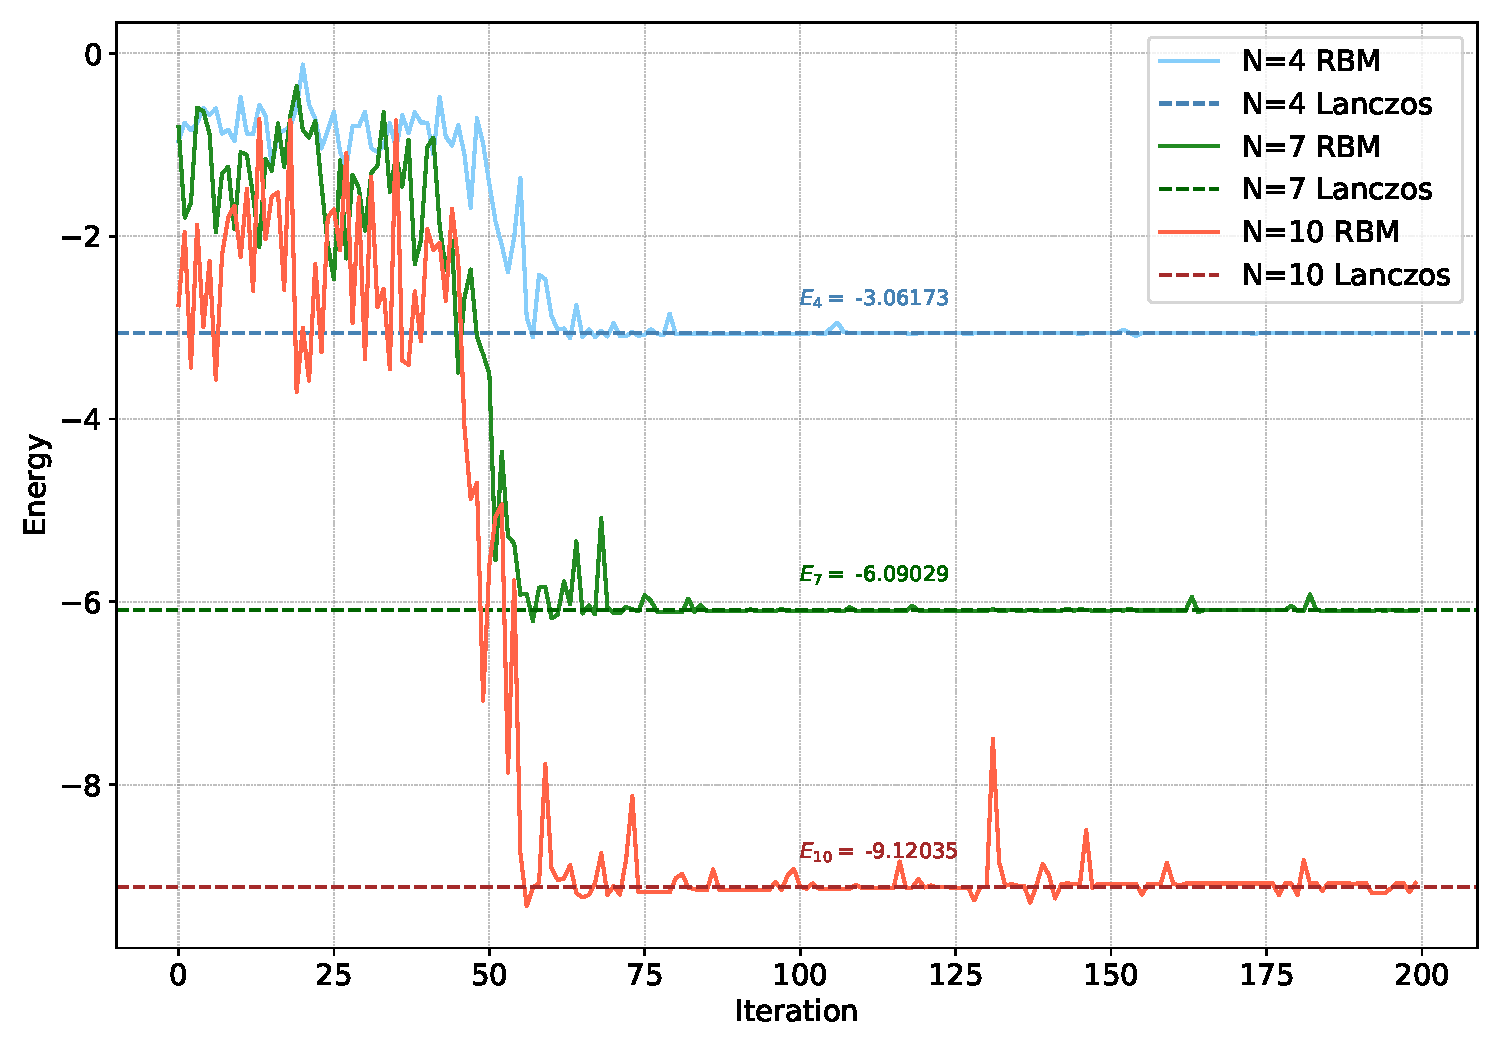
\includegraphics[width=0.85\textwidth]{./figure/Comparison_different_N.pdf}
\end{figure}

An import parameter of the RBM is the hidden unity density $\alpha$, that is the ratio between the number of hidden and visible neurons. Fig.~\ref{fig:comparison_alpha} shows the behavior of the RBM with $\alpha=2,4,6$ when describing a system with 7 spins. In our case, as displayed by Fig.~\ref{fig:normal}, we can reach the convergence to the right energy independently on the value of $\alpha$. However, even if the system is quite small, the difference with the Lanczos solution is overall smaller when $\alpha$ is bigger. This fact is presented in Fig.~\ref{fig:difference}, where these differences are enhanced using the log-scale. We can see that the orange line (corresponding to $\alpha=6$) reaches (at iteration 120-140) an accuracy between $10^{-3}$ and $10^{-4}$. It is to mention that $\alpha$ controls the complexity of the RBM, hence we expect that higher values of this parameter are needed when describing more complex systems, e.g. when the number of spins is larger.

\begin{figure}[htb]
    \centering 
    \caption{Performace of the RBM as function of the hidden unity density for a system with 7 spins described by a 1-dimensional Ising model in transverse field, without boundary conditions.}
    \label{fig:comparison_alpha}
    \begin{subfigure}[t]{0.45\textwidth}
        \centering
        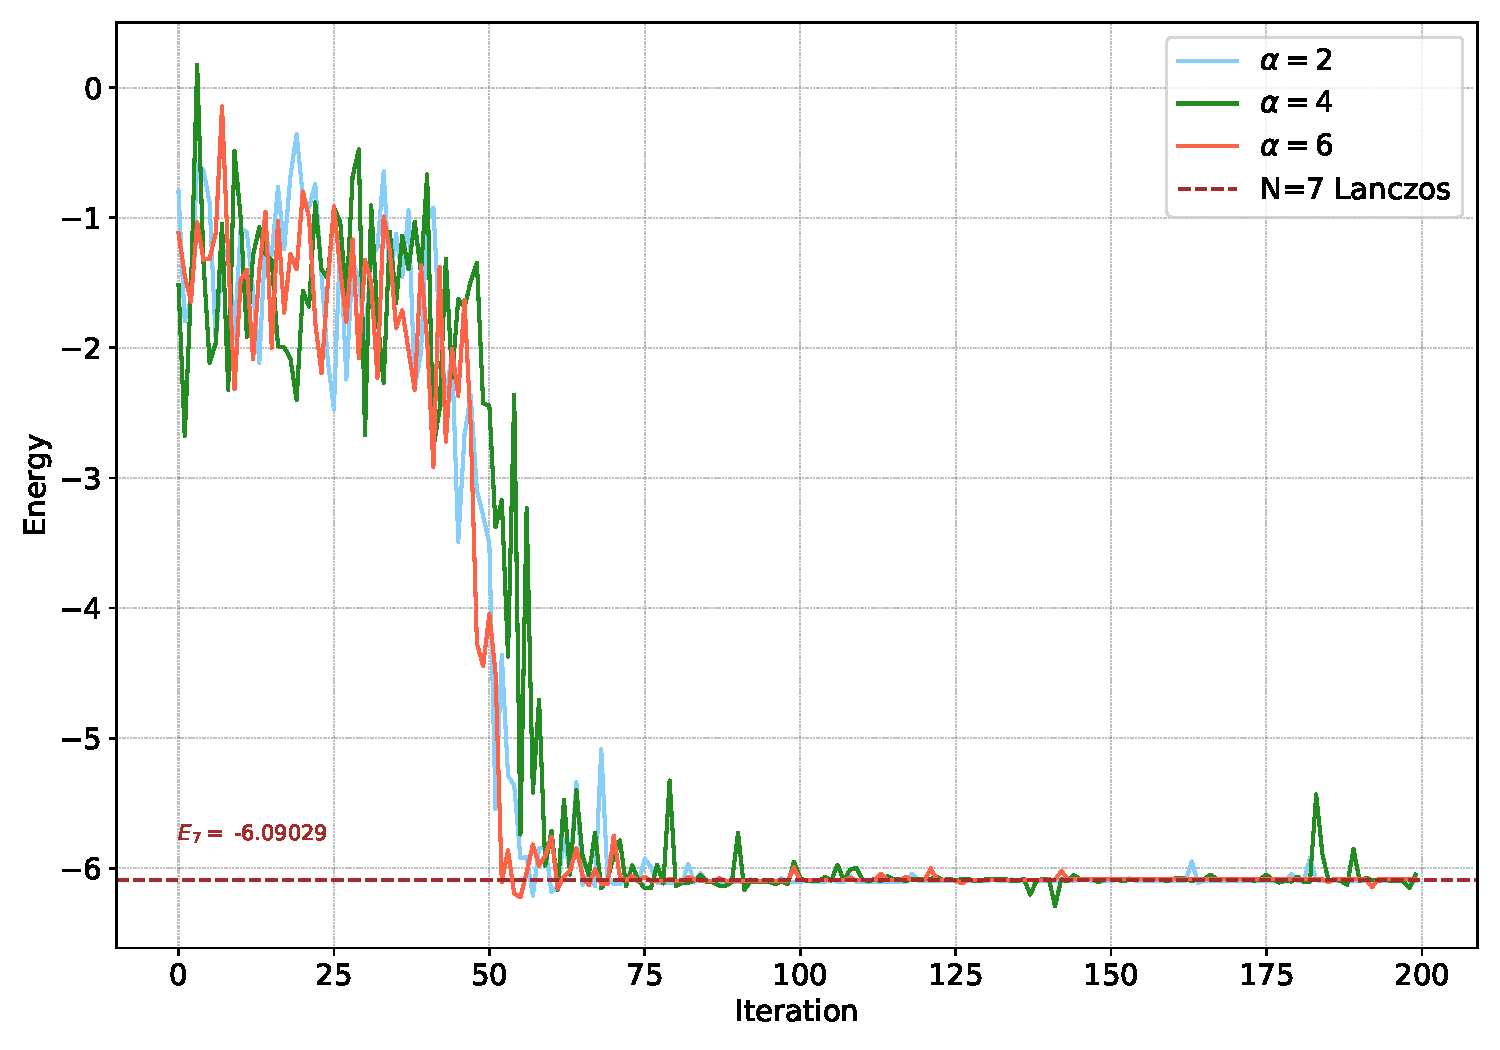
\includegraphics[width=\textwidth]{./figure/Comparison_energy_N_7_different_alpha.pdf}
        \caption{Predicted ground state energy for different vales of the hiddden unity density $\alpha$.}
        \label{fig:normal}
    \end{subfigure} 
    \begin{subfigure}[t]{0.45\textwidth} 
        \centering
        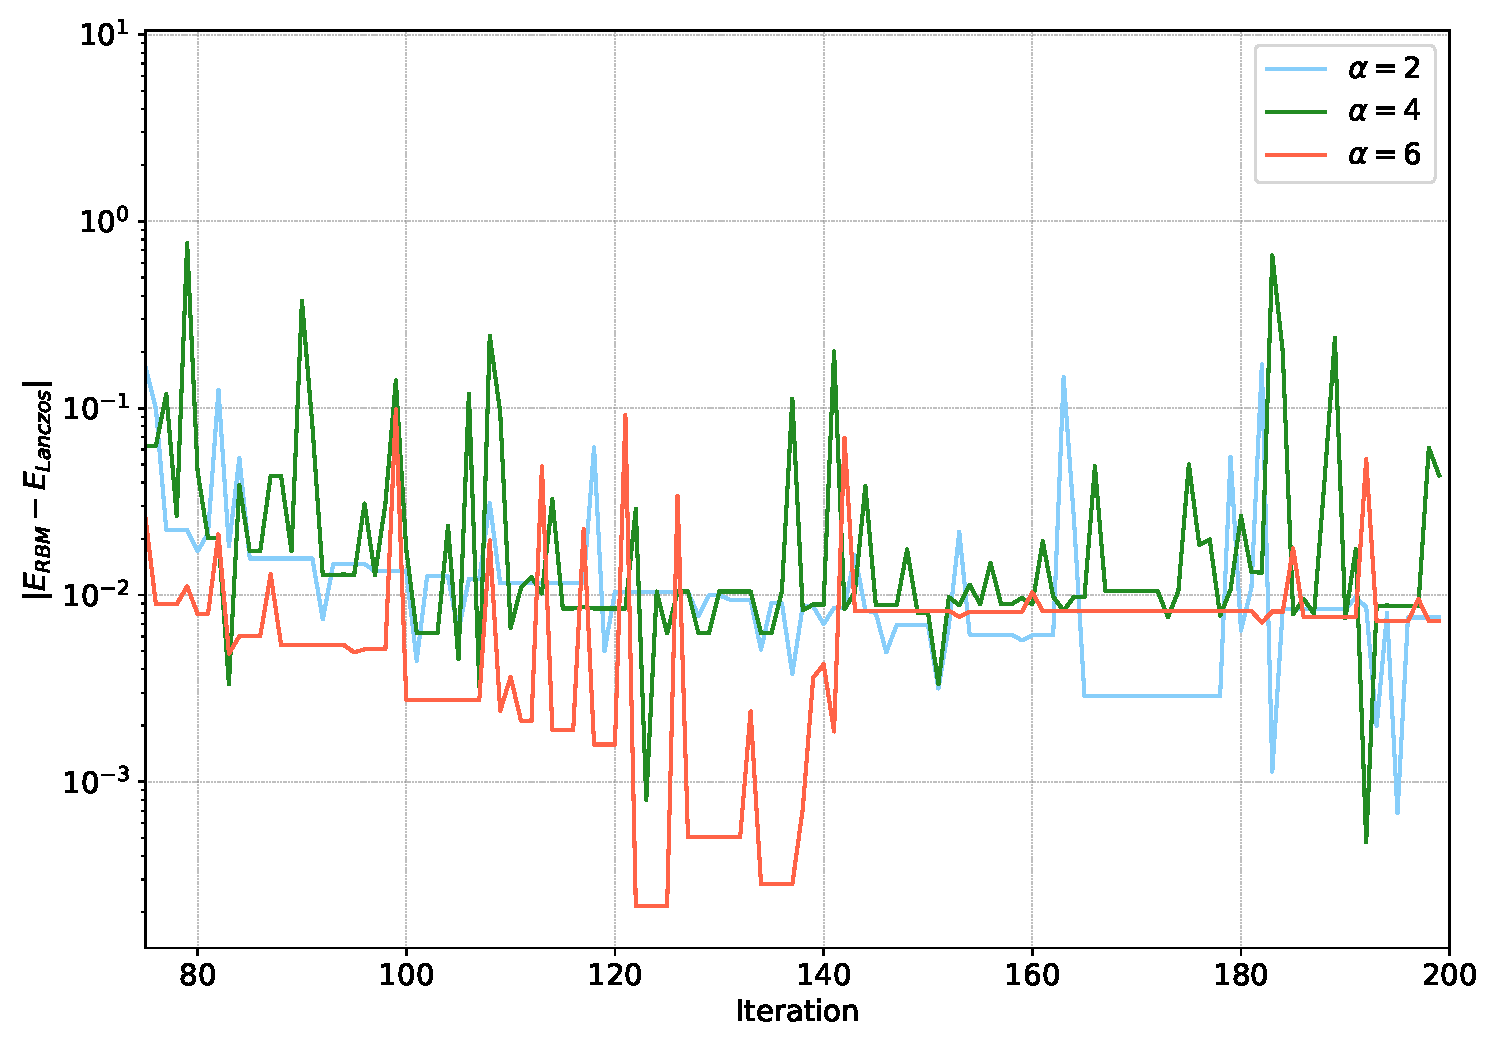
\includegraphics[width=\textwidth]{./figure/Comparison_N_7_different_alpha_difference_logscale.pdf}
        \caption{Differences between the ground state energy predicted by the RBM with and the true value given by the Lanczos algorithm; y-axis is in log-scale.}
        \label{fig:difference}
    \end{subfigure}
\end{figure}

\paragraph{2-dimensional Ising model}

The second application is the Ising model with transverse field in two dimensions. The hamiltonian of the system is the same of the 1-D case (Eq.~\ref{eq:ising}) with the difference that now the lattice is a 2-D square one with dimension $N = L^2$ and a given particle has neighbours not only at its left/right but also above and below itself. We still do not set boundary conditions. In our tests, the system has 9 spins in a $3 \times 3$ lattice. As for the 1-D cases, Fig.~\ref{fig:comparison_alpha_2D} shows the behaviour of the RBM during the training. Similar considerations as before can be made: the system oscillates a lot in the first part of the training ($\sim 50$ iterations), until it reaches convergence. We can distinguish a different response looking at Fig.~\ref{fig:difference_2D}. In this case we have that $\alpha =1$ reach the best value of accuracy (around $10^{-3}$) but using $\alpha = 4$ we get a more stable behaviour (e.g. better value of the mean of the accuracy).

\begin{figure}[htb]
    \centering 
    \caption{RBM ground state energy estimates for a system of 9 particles in a $3 \times 3$ square lattice, described by a transverse-field Ising model without boundary conditions.}
    \label{fig:comparison_alpha_2D}
    \begin{subfigure}[t]{0.45\textwidth}
        \centering
        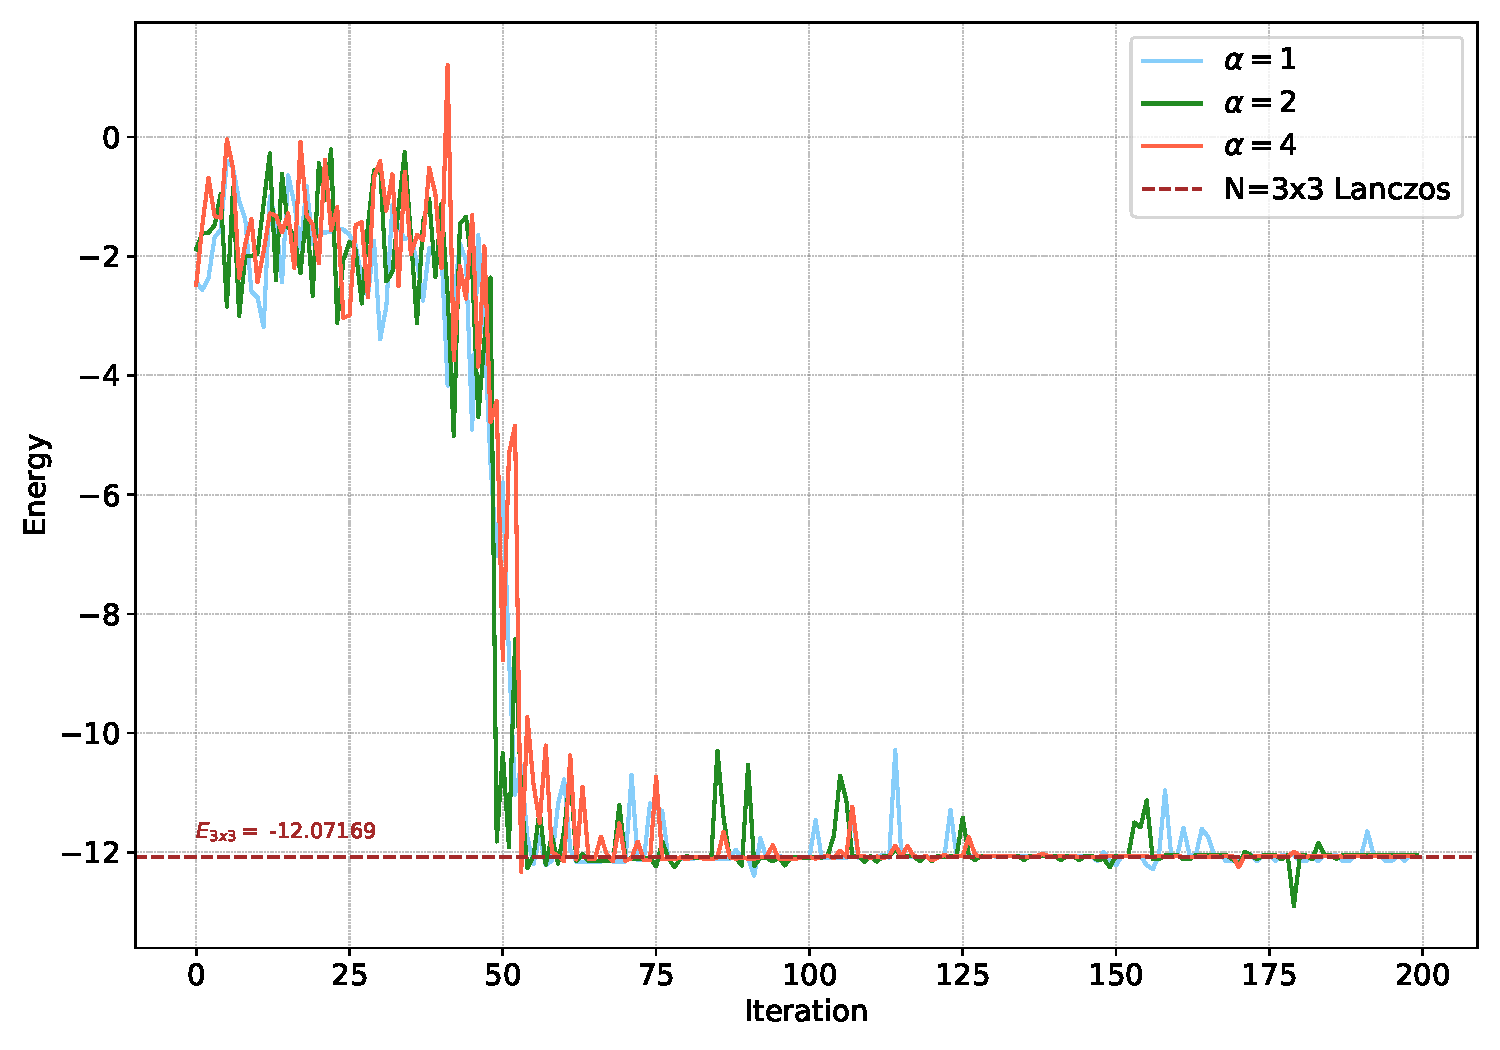
\includegraphics[width=\textwidth]{./figure/Comparison_energy_N_3x3_different_alpha.pdf}
        \caption{Ground state energy as function of the training iteration.}
        \label{fig:normal_2D}
    \end{subfigure} 
    \begin{subfigure}[t]{0.45\textwidth} 
        \centering
        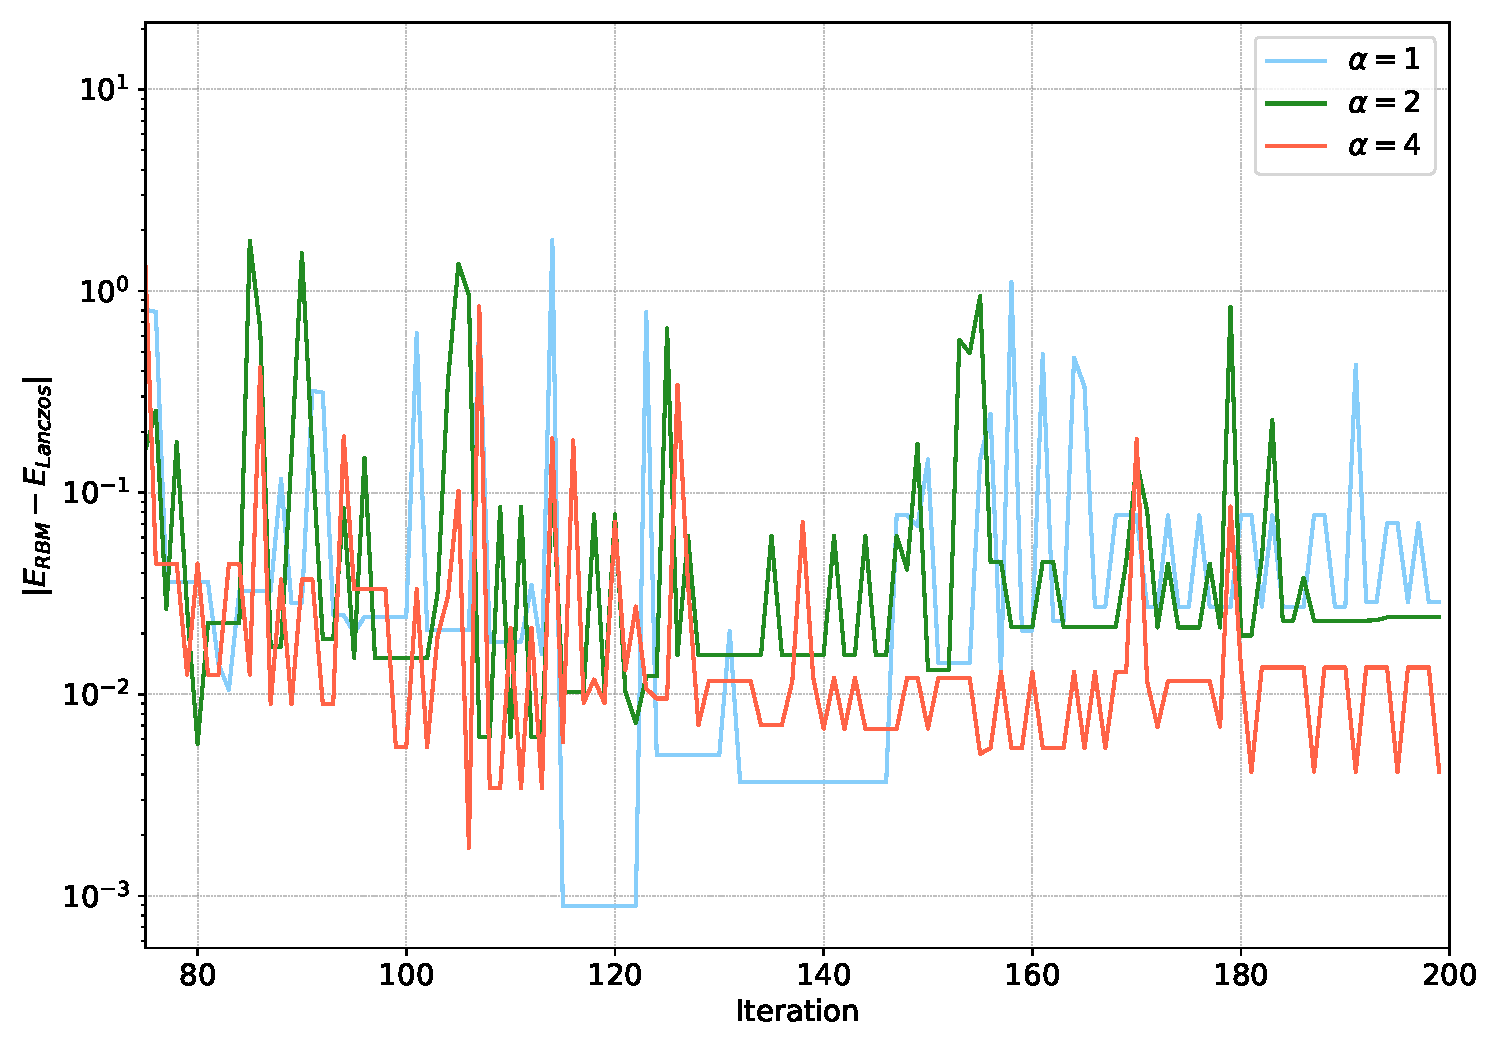
\includegraphics[width=\textwidth]{./figure/Comparison_N_3x3_different_alpha_difference_logscale.pdf}
        \caption{Differences between the ground state energy predicted by the RBM and the true value given by the Lanczos algorithm; y-axis is in log-scale.}
        \label{fig:difference_2D}
    \end{subfigure}
\end{figure}

\paragraph{NetKet implementation}

The most accurate implementation of neural networks description of a many-body quantum system can be obtained by the package NetKet\cite{netket}. It is build on C++ and features a Python interface. This paragraph provides a sight to the results that can be reached by state of the art implementation of neural networks quantum states.

Fig.~\ref{fig:alpha} shows the ground state energy for a $N=7$ particles system using different values of $\alpha$. If we compare this results against our algorithm (Fig.~\ref{fig:comparison_alpha}), we can see that NetKet is smoother and faster during the learning. This could be due to more complex regularization applied to the algorithm, that enhances numerical stability. Nevertheless, at equilibrium fluctuations are still present (even if this implementation is more stable), and the gain in accuracy with respect to our method is below a order of magnitude.

Netket is also optimized to work with systems with more than 14 particles; Fig.~\ref{fig:N} shows the behavior of the RBM using bigger values of $N$.

\begin{figure}[htb]
    \centering 
    \caption{NetKet RBM implementation results.}
    \label{fig:NetKet}
    \begin{subfigure}[t]{0.45\textwidth}
        \centering
        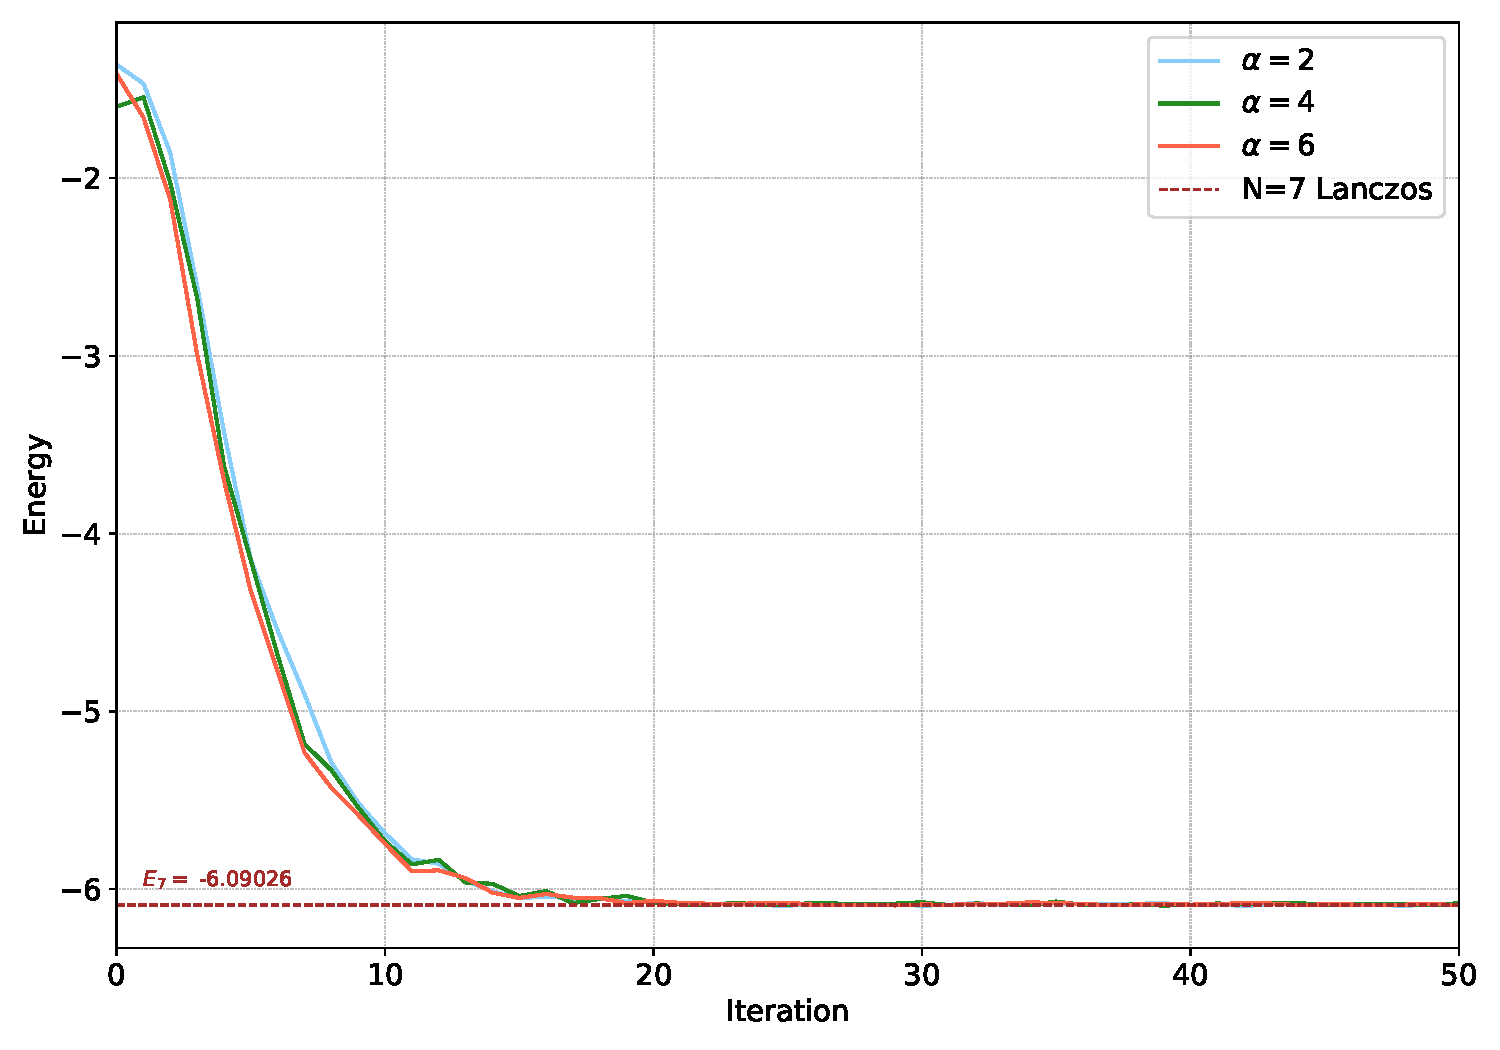
\includegraphics[width=\textwidth]{./figure/Comparison_energy_N_7_NetKet}
        \caption{Description of a system with 7 particles for different values of $\alpha$.}
        \label{fig:alpha}
    \end{subfigure} 
    \begin{subfigure}[t]{0.45\textwidth} 
        \centering
        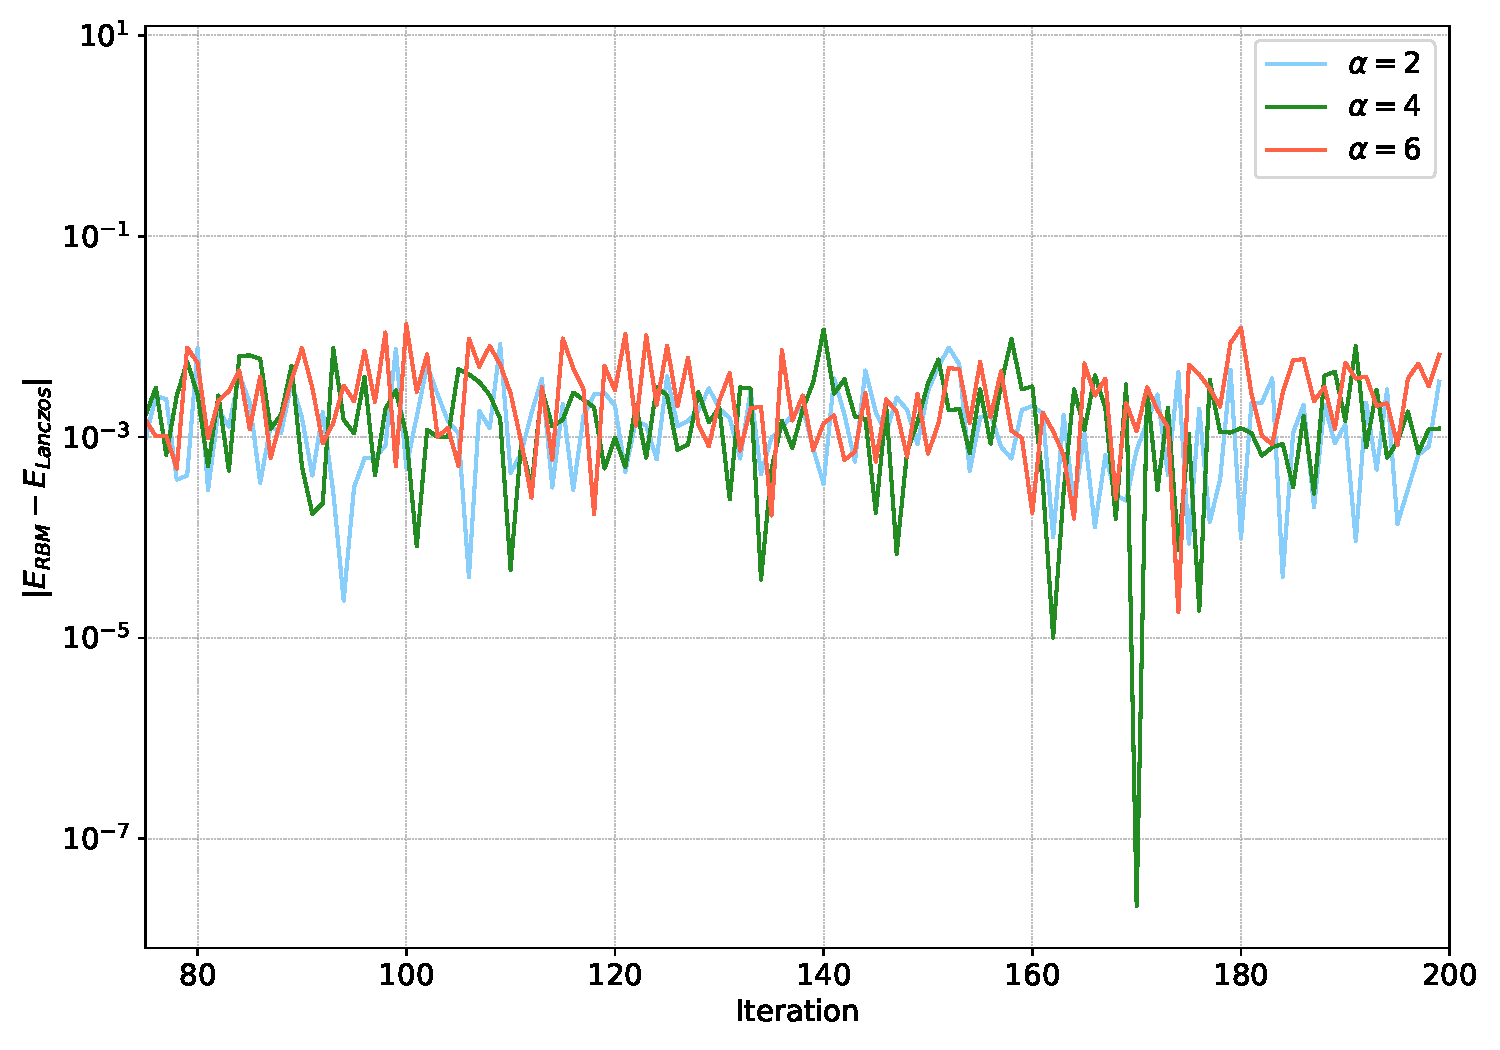
\includegraphics[width=\textwidth]{./figure/Comparison_N_7_difference_logscale_NET.pdf}
        \caption{Difference between the ground state energy predicted by RBM using NetKet and the true value by the Lanczos}
        \label{fig:Net_diff}
    \end{subfigure}
    \begin{subfigure}[t]{0.45\textwidth} 
        \centering
        \includegraphics[width=\textwidth]{./figure/Comparison_Net_Nostro.pdf}
        \caption{Difference between Lanczos solution and ground state energy obtained for a fixed $\alpha = 6$ using NetKet and our algorithm.}
        \label{fig:Net_nostro}
    \end{subfigure}
    \begin{subfigure}[t]{0.45\textwidth} 
        \centering
        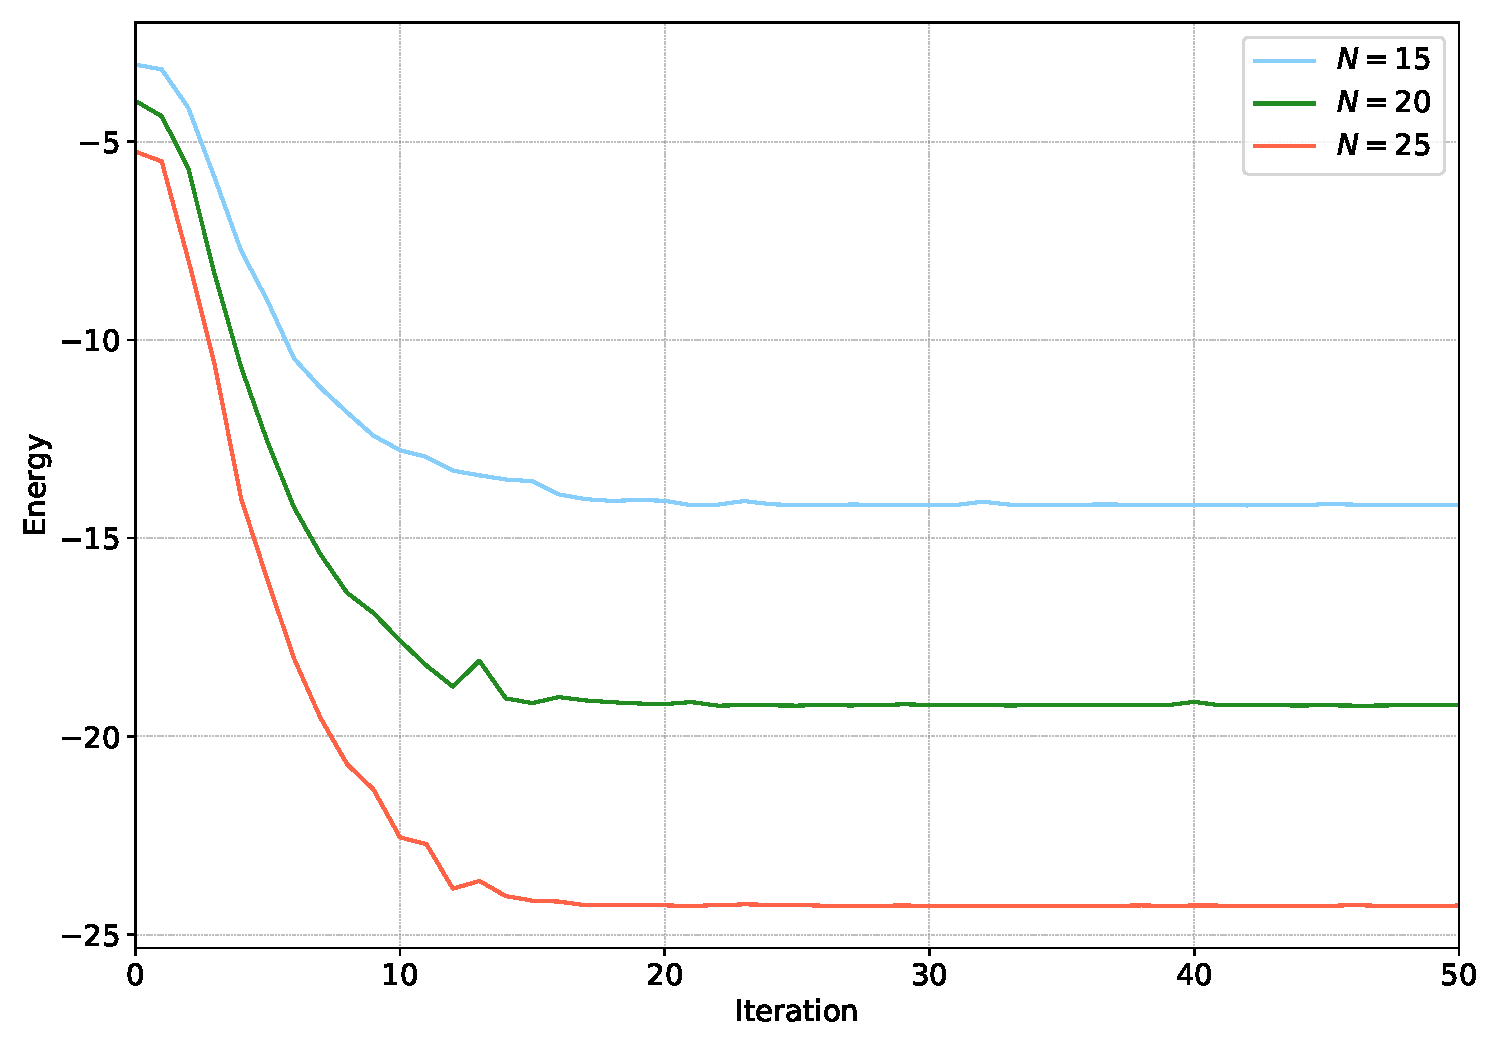
\includegraphics[width=\textwidth]{./figure/Comparison_NetKet.pdf}
        \caption{Ground state energy for system with larger amount of spins.}
        \label{fig:N}
    \end{subfigure}
    
\end{figure}

%%%%%%%%%%%%%%%%%%%%%%%%%%%%%%%%%%%%%%%%%%%%%%%%%%
%%%%%%%%%%%%%%%%%%%%%%%%%%%%%%%%%%%%%%%%%%%%%%%%%%
%%%%%%%%%%%%%%%%%%%%%%%%%%%%%%%%%%%%%%%%%%%%%%%%%%

\section{Conclusions and possible developments}
\label{sec:conclusion}

Machine learning techniques can be applied in the field of quantum many-body systems to solve problems such as the estimate of the ground state energy. This work focuses on the reproduction of a RBM as described in \cite{Carleo_2017}. 

As presented in Sec.~\ref{sec:results}, the implementation produces reasonable results in the description of the 1 and 2-dimensional Ising model in transverse field. The comparison against the solution provided by the Lanczos algorithm, shows an accuracy in the estimates the order of $10^{-2}$. This fact highlights that there is room for improvements, as confirmed by the state of the art implementation given by NetKet. 

In particular, regularizations to control the numerical stability should be investigated more in detail, since our results manifest the presence of noise that is absent in NetKet together with a slower convergence. Moreover, this point could be the main problem that afflicts the Fortran implementation and prevents it to reach the same results as the Python one (even if we are not able to precisely determine that, since the tested performed in Sec.~\ref{sec:test} did not supply clues on where the error can reside).

Another upgrade relies on the description of larger systems. The scripts developed only works up to 14 particles (in our machines with 8 Gb), since there is the need to keep in memory the matrix representation of the hamiltonian, that requires $2^N \times 2^N$ values to be stored if we are working with $N$ $1/2$-spins. This is actually not mandatory, since most elements of $H$ are equal to 0: hence sparse matrices can be a way to push forward this limit. An additional solution may even not require to store any elements of the matrix. In fact, we just need one element $H_{ij}$ at a time (see Sec.~\ref{sec:LocalEnergy}), so instead of calculate the whole matrix, we could compute just the element we need at demanding. 

An additional way to refine the results, could be to perform more run for each single system and mediate over the iteration; in this way we obtain a smoother behavior of the energy, since stochasticity is involved in the simulations.

%%%%%%%%%%%%%%%%%%%%%%%%%%%%%%%%%%%%%%%%%%%%%%%%%%
%%%%%%%%%%%%%%%%%%%%%%%%%%%%%%%%%%%%%%%%%%%%%%%%%%
%%%%%%%%%%%%%%%%%%%%%%%%%%%%%%%%%%%%%%%%%%%%%%%%%%

\bibliographystyle{IEEEtran}
{\footnotesize
\bibliography{references.bib}
}

%%%%%%%%%%%%%%%%%%%%%%%%%%%%%%%%%%%%%%%%%%%%%%%%%%
%%%%%%%%%%%%%%%%%%%%%%%%%%%%%%%%%%%%%%%%%%%%%%%%%%
%%%%%%%%%%%%%%%%%%%%%%%%%%%%%%%%%%%%%%%%%%%%%%%%%%

\clearpage

\begin{appendices}
%%%%%%%%%%%%%%%%%%%%%%%%%%%%%%%%%%%%%%%%%%%%%%%%%%
\section{Instability of Fortran implementation}
\label{appendix:fortran}

Fortran script does not provide stable results, even if each piece of code was tested against the counter part in Python (Sec.~\ref{sec:test}). Fig.~\ref{fig:fortran} clearly explains this problem: the results are obtained starting from the same conditions for a 1-dimensional system with 7 particles. It can be noticed that the covergens occurs at different values, and in some cases overflow leads to \texttt{NaN}.

\begin{figure}[htb]
    \centering
    \caption{Ground state energy predictions through Fortran implementation of the RBM for a system with 7 spins in 1-dimension. All the results are produced starting from the same conditions; hence clearly there is a problem of numerical stability.}
    \label{fig:fortran}
    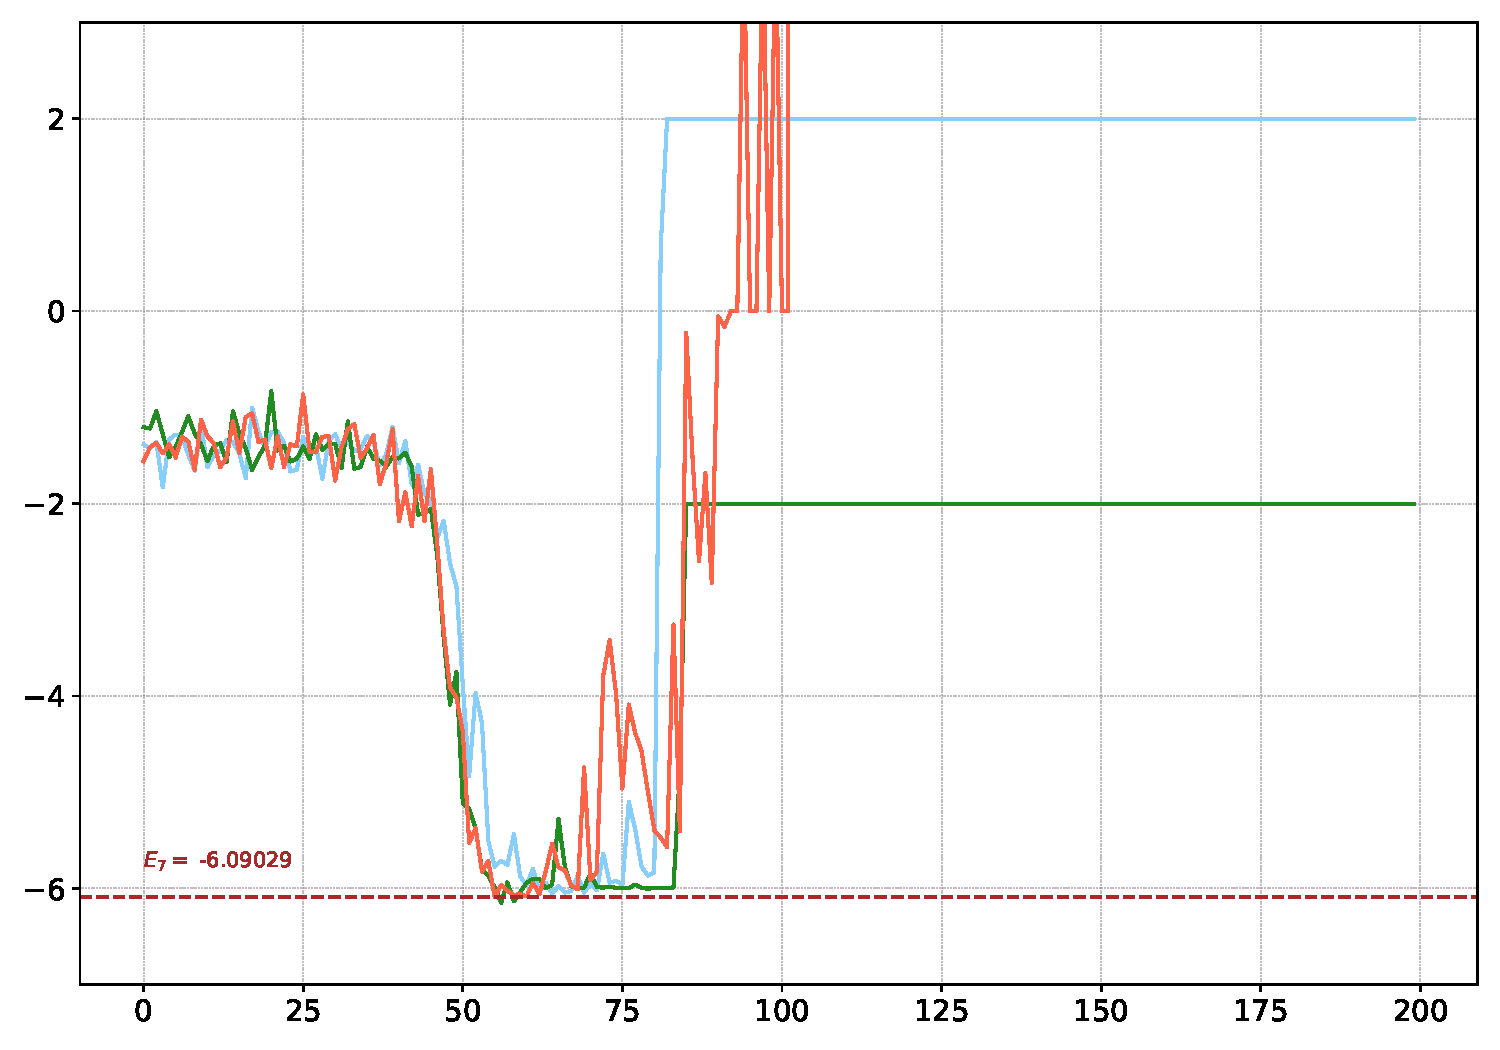
\includegraphics[width=.85\linewidth]{figure/fortran.pdf}
\end{figure}

%%%%%%%%%%%%%%%%%%%%%%%%%%%%%%%%%%%%%%%%%%%%%%%%%%
\section{Code Listings}
\label{appendix:code}

This appendix comprises the listings of code described in the report. In particular, the Fortran implementation is presented; the Python scripts follow the same logic and names, and they can be retrieved from the additional files delivered with the study.

Modules already developed during the classes or files that just gather the different functions to produce the results are not displayed here, but can be found in the support materials.

%%%%%%%%%%%%%%%%%%%%%%%%%%%%%%%%%%%%%%%%%%%%%%%%%%
\subsection{\texttt{simulation} module}

This module contains the subroutine to generate random configurations according to the current state of the RBM, using the acceptance rule of Eq.~\ref{eq:Metropolis}.

\lstinputlisting[language=Fortran, firstline=10, lastline=143, firstnumber=10, caption={Metropolis simulation subroutine to generate spin configurations from according to the state of the RBM.}, label={lst:Metropolis}]{Fortran/simulation.f90}

%%%%%%%%%%%%%%%%%%%%%%%%%%%%%%%%%%%%%%%%%%%%%%%%%%
\subsection{\texttt{rbm} module}

All the subroutine and functions that are needed to create and update the state of the RBM are included here.

\lstinputlisting[language=Fortran, firstline=9, lastline=68, firstnumber=9, caption={Random initialization of the parameters of the RBM (biases and weights).}, label={lst:RBM_init}]{Fortran/rbm.f90}

\lstinputlisting[language=Fortran, firstline=70, lastline=146, firstnumber=70, caption={RBM weights update subroutine (Eq.~\ref{eq:update}).}, label={lst:RBM_update}]{Fortran/rbm.f90}

\lstinputlisting[language=Fortran, firstline=148, lastline=230, firstnumber=148, caption={Covariance matrix (Eq.\ref{eq:cov_mat}).}, label={lst:Skk}]{Fortran/rbm.f90}

\lstinputlisting[language=Fortran, firstline=132, lastline=300, firstnumber=132, caption={Forces vector calculation (Eq.~\ref{eq:forces}).}, label={lst:Forces}]{Fortran/rbm.f90}

\lstinputlisting[language=Fortran, firstline=302, lastline=408, firstnumber=302, caption={Local energy derivation from a set of spin configurations (Eq.\ref{eq:Eloc}).}, label={lst:LocalEnergy}]{Fortran/rbm.f90}

%%%%%%%%%%%%%%%%%%%%%%%%%%%%%%%%%%%%%%%%%%%%%%%%%%
\subsection{\texttt{random} module}

Small set of functions to provide random number in different contexts from the uniform distribution.

\lstinputlisting[language=Fortran, firstline=7, lastline=56, firstnumber=7, caption={Random number from normal distribution.}, label={lst:Random_Normal}]{Fortran/random.f90}

\lstinputlisting[language=Fortran, firstline=58, lastline=94, firstnumber=58, caption={Random integer number.}, label={lst:Random_Integer}]{Fortran/random.f90}

\lstinputlisting[language=Fortran, firstline=96, lastline=130, firstnumber=96, caption={Random spin configuration.}, label={lst:Random_Configuration}]{Fortran/random.f90}

%%%%%%%%%%%%%%%%%%%%%%%%%%%%%%%%%%%%%%%%%%%%%%%%%%
\subsection{\texttt{others} module}

Routines needed to perform auxiliary tasks.

\lstinputlisting[language=Fortran, firstline=7, lastline=41, firstnumber=7, caption={Integer representation of a spin configuration.}, label={lst:idx_from_config}]{Fortran/others.f90}

\lstinputlisting[language=Fortran, firstline=43, lastline=96, firstnumber=43, caption={Spin configuration from its integer representation.}, label={lst:config_from_idx}]{Fortran/others.f90}

\lstinputlisting[language=Fortran, firstline=100, lastline=148, firstnumber=100, caption={Integer conversion to its binary representation.}, label={lst:int2bit}]{Fortran/others.f90}

\lstinputlisting[language=Fortran, firstline=150, lastline=221, firstnumber=150, caption={Logarithm of the ration between two wave wave functions $\Psi_M(S_2)$ and $\Psi_M(S_1)$.}, label={lst:logPsiDiff}]{Fortran/others.f90}

\lstinputlisting[language=Fortran, firstline=223, lastline=278, firstnumber=223, caption={Inverse of a square matrix.}, label={lst:Inverse}]{Fortran/others.f90}

%%%%%%%%%%%%%%%%%%%%%%%%%%%%%%%%%%%%%%%%%%%%%%%%%%
\subsection{\texttt{Lanczos\_mod} module}

Lanczos subroutine is used to retrieve the correct solution given the hamiltonian of a system.

\lstinputlisting[language=Fortran, firstline=7, lastline=161, firstnumber=7, caption={Lanczos algorithm.}, label={lst:Lanczos}]{Fortran/Lanczos.f90}

%%%%%%%%%%%%%%%%%%%%%%%%%%%%%%%%%%%%%%%%%%%%%%%%%%
\subsection{Python interface to Fortran}
The script through which Fortran code should be called is presented here.

\lstinputlisting[language=Python, caption={Python interface to Fortran code.}, label={lst:run}]{Fortran/run.py}

%%%%%%%%%%%%%%%%%%%%%%%%%%%%%%%%%%%%%%%%%%%%%%%%%%
\subsection{Test script and results between Fortran and Python}

The test script used to check Fortran code against the Python implementation is presented here, along with the full output.

\lstinputlisting[language=Fortran, caption={Script for testing the correctness of the code}, label={lst:test}]{Fortran/test.f90}

\lstinputlisting[caption={Results of the test produced by Fortran code}, label={lst:test_fortran}]{Fortran/test.txt}

\lstinputlisting[caption={Results of the test produced by Python code}, label={lst:test_python}]{Python/test.txt}

\end{appendices}

%%%%%%%%%%%%%%%%%%%%%%%%%%%%%%%%%%%%%%%%%%%%%%%%%%
%%%%%%%%%%%%%%%%%%%%%%%%%%%%%%%%%%%%%%%%%%%%%%%%%%
%%%%%%%%%%%%%%%%%%%%%%%%%%%%%%%%%%%%%%%%%%%%%%%%%%

\end{document}
